\documentclass[letterpaper,11pt]{article}

\usepackage[spanish,es-tabla]{babel}
\usepackage[utf8]{inputenc}
\usepackage[T1]{fontenc}
\usepackage{lmodern}
\usepackage[top=1.7cm,bottom=1.9cm,left=2.2cm,right=2.2cm,headheight=28pt,includehead,headsep=0.5cm]{geometry}
\usepackage{graphicx}
\usepackage{xcolor}
\usepackage{booktabs}
\usepackage{array}
\usepackage{float}
\usepackage{enumitem}
\usepackage{fancyhdr}
\usepackage{hyperref}
\usepackage{amsmath}
\usepackage{amssymb}
\usepackage{tikz}
\usetikzlibrary{positioning,arrows.meta}
\usepackage{caption}
\usepackage{listings}

\definecolor{verde}{RGB}{0,128,0}
\definecolor{azulmarino}{RGB}{0,0,128}
\definecolor{gris}{RGB}{95,95,95}
\hypersetup{colorlinks=true,linkcolor=azulmarino,urlcolor=azulmarino,citecolor=azulmarino}

\lstset{basicstyle=\ttfamily\footnotesize,breaklines=true,frame=single,
  backgroundcolor=\color{gris!8},columns=fullflexible,keepspaces=true,
  numbers=none,xleftmargin=4pt,xrightmargin=4pt,aboveskip=6pt,belowskip=6pt}

\newcommand{\universidad}{Universidad Técnica Metropolitana}
\newcommand{\codcurso}{INF8090}
\newcommand{\nombrecurso}{Computación Paralela y Distribuida}
\newcommand{\carrera}{Ingeniería Civil en Ciencia de Datos}
\newcommand{\profesor}{Dr. Ing. Michael Miranda Sandoval}

\fancyhf{}
\fancyheadoffset[L]{0.4cm}
\fancyhead[L]{
\begin{tikzpicture}[remember picture,overlay]
    \fill[verde] (current page.north west) rectangle ++(\paperwidth/3,-0.18cm);
    \fill[azulmarino] ([xshift=\paperwidth/3]current page.north west) rectangle ++(\paperwidth*2/3,-0.18cm);
    \fill[azulmarino] (current page.south west) rectangle ++(\paperwidth*0.75,0.18cm);
    \fill[verde] ([xshift=0.75\paperwidth]current page.south west) rectangle ++(\paperwidth*0.25,0.18cm);
\end{tikzpicture}
\rmfamily \fontsize{9}{11}\selectfont
{\textcolor{verde}{\codcurso} - \textcolor{azulmarino}{\nombrecurso}\\
\textcolor{gris}{\carrera}}}
\fancyfoot[C]{\fontsize{7pt}{7pt}\selectfont \color{gris}
    \universidad\ - Proyecto Semestral \hfill \thepage}
\renewcommand{\headrulewidth}{0pt}
\renewcommand{\footrulewidth}{0.05pt}
\setlength{\parskip}{0.35em}

\begin{document}
\pagestyle{fancy}
\shorthandoff{<>}   % spanish babel hace activos < y > (guillemets); rompen las flechas -> de TikZ

% ===================== 1. PORTADA =====================
\begin{center}
{\Large\bfseries Detección distribuida de anomalías de comportamiento en trayectorias ADS-B\par}
\vspace{0.15cm}
{\large\itshape mediante un orquestador de tareas propio (coordinador--agentes) evaluado en local y en un clúster QEMU\par}
\vspace{0.35cm}
\begin{tabular}{rl}
\textbf{Integrantes:} & Welinton Barrera Mondaca \quad (\texttt{wbarrera@utem.cl}) \\
 & Joaquín Ignacio Araya Bustos \quad (\texttt{jarayabu@utem.cl}) \\
 & Juan Cristóbal Toledo Fierro \quad (\texttt{jtoledof@utem.cl}) \\
\textbf{Profesor:} & \profesor \\
\textbf{Curso / Sección:} & \codcurso\ -- \nombrecurso\ / 412 \\
\textbf{Fecha:} & Julio de 2026 \\
\end{tabular}
\end{center}
\vspace{0.1cm}\hrule\vspace{0.25cm}

% ===================== 2. RESUMEN EJECUTIVO =====================
\section*{Resumen ejecutivo}
Se aborda la \textbf{detección no supervisada de anomalías de comportamiento} (rodeos, esperas
prolongadas, descensos anómalos y aproximaciones interrumpidas) en trayectorias de vuelo reales
obtenidas de \textbf{OpenSky Network} (ADS-B). La etapa de \emph{scoring} de anomalías es
\emph{embarrassingly-parallel} sobre particiones de vuelos, lo que justifica una solución
\textbf{distribuida}. Se implementó un \textbf{orquestador de tareas propio} (coordinador + agentes con
paso de mensajes por TCP, cola dinámica de trabajo y tolerancia a fallos) y una tarea enchufable de
detección basada en un puntaje \textbf{$z$-robusto (MAD)}. La evaluación experimental, con línea base
secuencial y repeticiones, muestra un \textbf{speedup de $S_p=5{,}59$ con $p=8$ nodos} (eficiencia
$E_p=0{,}70$) sobre una carga con cómputo denso, y una \textbf{calidad de detección de recall $=1{,}0$}
sobre anomalías inyectadas para validar, además de encontrar 8 vuelos reales genuinamente anómalos. Se
concluye que el patrón de particionamiento escala de forma predecible y que la \emph{granularidad} es la
variable determinante: la variante sobre datos reales de bajo volumen es \emph{I/O-bound} y no acelera,
un resultado esperado que se documenta con rigor.

% ===================== 3. INTRODUCCION =====================
\section{Introducción y motivación}
Las aeronaves comerciales emiten continuamente su estado (posición, altitud, velocidad, rumbo) mediante
\textbf{ADS-B}. Dentro del tráfico normal existen trayectorias con desviaciones sistemáticas respecto del
patrón esperado: maniobras evasivas, \emph{go-arounds}, \emph{holdings} prolongados, descensos anómalos o
cambios de rumbo no compatibles con la ruta. Se consideran cuatro tipos:
\begin{itemize}[nosep,leftmargin=1.3em]
  \item \textbf{Rodeo}: desvío lateral notable respecto de la ruta directa origen--destino.
  \item \textbf{Holding}: patrón de espera (bucles) prolongado.
  \item \textbf{Descenso anómalo}: pérdida de altitud pronunciada e inusual para la fase de vuelo.
  \item \textbf{Go-around}: aproximación interrumpida (descenso seguido de reascenso).
\end{itemize}
Detectar y \textbf{rankear} estas anomalías es pertinente para ciencia de datos: habilita análisis de
seguridad operacional, auditoría de eficiencia de rutas y caracterización de tráfico no rutinario.

El problema no es de ingeniería plana porque exige \emph{feature engineering} de comportamiento no
trivial y un modelo de \emph{outlier scoring} robusto. La \textbf{justificación del paralelismo} es
concreta: el \emph{scoring} es independiente por vuelo (o por partición de vuelos), de modo que una vez
extraídas las \emph{features} el cálculo se reparte sin dependencias entre trozos. A volúmenes grandes,
una solución secuencial no termina en tiempo razonable; la escala es lo que motiva distribuir.

% ===================== 4. OBJETIVOS =====================
\section{Objetivo general y objetivos específicos}
\textbf{Objetivo general:} diseñar, implementar y evaluar una solución \textbf{distribuida} que detecte y
rankee anomalías de comportamiento en trayectorias ADS-B, con una justificación técnica real del uso de
distribución.

\textbf{Objetivos específicos:}
\begin{itemize}[nosep,leftmargin=1.3em]
  \item Construir una \textbf{línea base secuencial} comparable (mismo problema, mismos datos).
  \item Implementar un \textbf{orquestador coordinador--agentes} con particionamiento, cola dinámica,
        comunicación por TCP, reducción y tolerancia a fallos.
  \item Medir \textbf{speedup, eficiencia y overhead} variando el número de nodos $p$, con repeticiones.
  \item Evaluar la \textbf{calidad} de la detección (recall sobre anomalías inyectadas) sobre datos reales.
  \item Realizar un \textbf{análisis crítico} honesto (granularidad, overhead, cuellos de botella).
\end{itemize}

% ===================== 5. DATOS =====================
\section{Datos utilizados}
\textbf{Origen y estructura.} Se emplean vuelos reales de \textbf{OpenSky Network} (endpoint
\texttt{/states/all}, acceso anónimo). De cada vector de estado se usan \texttt{icao24}, \texttt{callsign},
\texttt{lat}, \texttt{lon} y \texttt{baroaltitude}. Un proceso de ingesta (\texttt{ingesta\_adsb.py})
realiza \emph{polling} sobre un \emph{bounding box} (Europa central, alto tráfico), agrupa los estados por
\texttt{icao24} en trayectorias, filtra las de menos de 8 puntos y \textbf{resamplea} cada vuelo a 40
puntos $[\text{lat},\text{lon},\text{alt}]$. En la corrida reportada se capturaron \textbf{636 vuelos
reales} ($\approx$732 KB en JSON), incluidos en el repositorio.

\begin{table}[H]\centering\small
\caption{Esquema de una trayectoria tras la ingesta y \emph{features} de comportamiento derivadas.}
\label{tab:esquema}
\begin{tabular}{lll}
\toprule
Campo / \emph{feature} & Tipo & Uso \\
\midrule
\texttt{icao24} & texto & identificador único de la aeronave (agrupación) \\
\texttt{callsign} & texto & indicativo de vuelo (etiqueta legible) \\
\texttt{track}[40] & $[\text{lat},\text{lon},\text{alt}]$ & trayectoria resampleada a 40 puntos \\
\midrule
\texttt{len\_ratio} & real & largo real (\emph{haversine}) / distancia directa: desvío de ruta \\
\texttt{turn\_sum} & real & suma de cambios de rumbo: curvatura acumulada \\
\texttt{vrate\_max} & real & tasa vertical máxima: descensos/ascensos anómalos \\
\bottomrule
\end{tabular}
\end{table}

\textbf{Ground truth y evaluación híbrida.} Como el \emph{ground truth} real es escaso, se sigue una
\textbf{evaluación híbrida}: sobre vuelos reales rectos se \textbf{inyectan anomalías controladas}
(perturbaciones deterministas de ruta o altitud) que permiten medir \textbf{recall}, y en paralelo se
reportan los vuelos reales que el detector marca como más anómalos (hallazgos).

\textbf{Datos sintéticos por semilla.} Para el estudio de escalabilidad se usa una carga con cómputo denso
generada por \emph{datos-por-semilla}: cada partición transporta únicamente una \textbf{semilla} y
parámetros; el agente \textbf{regenera} sus trayectorias con \texttt{random.Random(seed)} dentro de
\texttt{run()}. Esto es reproducible (semilla fija) y logra \textbf{transferencia de datos $\approx$ cero},
aislando el costo de cómputo del de comunicación.

% ===================== 6. LINEA BASE =====================
\section{Línea base}
La referencia secuencial (\texttt{baseline\_seq.py}) ejecuta el mismo contrato de tarea
(\texttt{split/run/merge}) en \textbf{un solo proceso}, sin red, y mide el tiempo de pared $T_1$. Es
determinista (semilla $=7$) y produce \textbf{exactamente el mismo resultado} que la versión distribuida:
esta \textbf{equivalencia} se verifica automáticamente en cada corrida (comparación del ranking
\emph{top-k} y de las métricas), condición necesaria para poder reportar \emph{speedup} según la
advertencia metodológica de la pauta.

\textbf{Verificación de equivalencia.} La comparación no es informal: tras cada corrida distribuida se
contrastan, elemento a elemento, el \textbf{ranking top-k} (identidad de los vuelos y su orden) y las
\textbf{métricas agregadas} (recall, precision@k, conteos TP/FP) contra la línea base con la misma semilla.
Si difirieran, el \emph{speedup} no se reportaría. Esta disciplina evita el error habitual de comparar los
tiempos de dos programas que en realidad calculan cosas distintas, y hace que $T_1$ y $T_p$ sean
estrictamente comparables: la única diferencia entre ambas ejecuciones es \textbf{cómo} se reparte el
cómputo, no \textbf{qué} se calcula.

% ===================== 7. DISENO =====================
\section{Diseño de la solución}
\textbf{Arquitectura.} Un \textbf{coordinador} en el host reparte trabajo a $N$ \textbf{agentes}
(\texttt{worker\_agent.py}) por \textbf{TCP}, serializando un JSON por línea (recepción acumulada en
\emph{buffers} de 64 KB). La plataforma es \textbf{agnóstica al dominio}: la lógica ADS-B vive en una
\textbf{tarea enchufable} que implementa un contrato mínimo:

\begin{lstlisting}[language=Python]
def split(payload, workers): -> [chunk, ...]   # particiona el problema
def run(chunk):              -> parcial         # procesa una particion (en el agente)
def merge(parciales):        -> resultado       # reduccion global (ranking top-k)
def self_test():             -> (chunk, esperado)  # sonda de salud funcional
\end{lstlisting}

\begin{figure}[H]\centering
\begin{tikzpicture}[font=\small,
  box/.style={draw,rounded corners,minimum height=9mm,minimum width=30mm,align=center},
  ag/.style={draw,rounded corners,minimum height=8mm,minimum width=20mm,align=center,fill=verde!8}]
  \node[box,fill=azulmarino!10] (coord) {\textbf{Coordinador} (host)\\cola dinámica de trabajo};
  \node[ag,below left=12mm and 8mm of coord] (a1) {agente\\nodo1};
  \node[ag,below=12mm of coord] (a2) {agente\\nodo2};
  \node[ag,below right=12mm and 8mm of coord] (a3) {agente\\$\ldots$};
  \draw[->] (coord) -- node[left,pos=.5,font=\scriptsize]{tarea} (a1);
  \draw[->] (coord) -- (a2);
  \draw[->] (coord) -- node[right,pos=.5,font=\scriptsize]{tarea} (a3);
  \draw[->,dashed] (a1) to[bend left=18] node[left,font=\scriptsize,pos=.6]{resultado} (coord);
  \draw[->,dashed] (a3) to[bend right=18] (coord);
\end{tikzpicture}
\caption{Orquestador coordinador--agentes. \texttt{split} reparte trozos por TCP desde una cola dinámica;
cada agente ejecuta \texttt{run} en paralelo (línea continua = tarea, discontinua = resultado);
\texttt{merge} reduce los parciales en el ranking global.}
\label{fig:arq}
\end{figure}

\textbf{Particionamiento y granularidad.} \texttt{split()} divide el problema en \texttt{n\_chunks}
trozos independientes (subconjuntos de vuelos, o semilla+parámetros en el caso sintético). El número de
trozos controla la \textbf{granularidad}: trozos grandes reducen el \emph{overhead} de coordinación pero
limitan el balanceo; trozos pequeños balancean mejor pero la comunicación puede dominar.

\textbf{Cola dinámica y balanceo.} El coordinador mantiene una \textbf{cola de trabajo}; cada agente que
queda libre solicita el siguiente trozo (\emph{work-stealing} implícito). Así el reparto se adapta a la
velocidad real de cada nodo, sin asignación estática (Figura~\ref{fig:seq}).

\textbf{Sincronización y reducción.} No hay dependencias entre trozos (paralelismo de datos puro); el
único punto de sincronización es la \textbf{reducción} final: \texttt{merge()} fusiona los parciales y
produce el \textbf{ranking top-k global} de los vuelos más anómalos.

\textbf{Protocolo de comunicación.} El intercambio coordinador$\leftrightarrow$agente usa
\textbf{mensajes JSON delimitados por línea} sobre TCP; el receptor acumula en un \emph{buffer} de 64~KB y
separa por \texttt{\textbackslash n}, tolerando mensajes fragmentados en varios segmentos. Los tipos son:

\begin{table}[H]\centering\small
\caption{Tipos de mensaje del protocolo coordinador--agente.}
\label{tab:proto}
\begin{tabular}{lll}
\toprule
Mensaje & Sentido & Contenido \\
\midrule
\texttt{HELLO} / \texttt{SELFTEST} & coord.\ $\to$ agente & despliegue y sonda de salud (\texttt{self\_test}) \\
\texttt{TASK} & coord.\ $\to$ agente & un trozo (subconjunto de vuelos o semilla+parámetros) \\
\texttt{RESULT} & agente $\to$ coord. & parcial (\emph{top} local + conteos) \\
\texttt{ERROR} / \emph{timeout} & agente $\to$ coord. & fallo del trozo $\Rightarrow$ reintento o exclusión \\
\bottomrule
\end{tabular}
\end{table}

\begin{figure}[H]\centering
\begin{tikzpicture}[font=\footnotesize,>={Latex[length=2mm]}]
  \node[font=\small\bfseries] (C) at (0,0) {Coordinador};
  \node[font=\small\bfseries] (A) at (7,0) {Agente};
  \draw[gris,dashed] (0,-0.35) -- (0,-4.4);
  \draw[gris,dashed] (7,-0.35) -- (7,-4.4);
  \draw[->] (0,-0.8) -- node[above,font=\scriptsize]{\texttt{TASK}(chunk $i$)} (7,-0.8);
  \node[draw,rounded corners,fill=verde!10,minimum width=2.4cm,minimum height=6mm] at (7,-1.6) {\texttt{run(chunk)}};
  \draw[->,dashed] (7,-2.4) -- node[above,font=\scriptsize]{\texttt{RESULT}(parcial $i$)} (0,-2.4);
  \draw[->] (0,-3.1) -- node[above,font=\scriptsize]{\texttt{TASK}(chunk $i{+}1$)} (7,-3.1);
  \node[text=gris,font=\scriptsize] at (3.5,-4.1) {si el trozo falla o el nodo cae: reintento o exclusión, sin detener el \emph{job}};
\end{tikzpicture}
\caption{Ciclo de una unidad de trabajo: el coordinador reparte un trozo (\texttt{TASK}), el agente lo
procesa (\texttt{run}) y devuelve el parcial (\texttt{RESULT}); al quedar libre recibe el siguiente. El
reparto es dinámico y degrada con gracia ante fallos.}
\label{fig:seq}
\end{figure}

\textbf{Tolerancia a fallos.} Antes de trabajar, cada nodo pasa un \emph{health-check} funcional
(\texttt{self\_test}: se compara su salida contra la esperada). Durante la ejecución, un trozo que falla
se \textbf{reintenta} o se \textbf{abandona} sin detener el job; un nodo que cae se \textbf{excluye} y el
resto completa el trabajo. Esto se demostró en el clúster: con un nodo inicialmente inalcanzable, el job
terminó $8/8$ en el nodo sano.

\textbf{Modos de ejecución.} (i) \textbf{Local}: los agentes son \textbf{procesos} separados en el host,
lo que \textbf{evita el GIL} y permite cómputo real en paralelo (equivalente a \emph{multiprocessing}
sobre sockets). (ii) \textbf{Clúster QEMU}: los agentes corren en VMs Debian; el coordinador despliega el
agente y la tarea por SSH/SFTP y los alcanza por puertos reenviados.

\textbf{Detección (dominio).} De cada trayectoria se extraen tres \emph{features}: \emph{desvío de ruta}
(\texttt{len\_ratio}, largo real vía \emph{haversine} sobre la distancia directa), \emph{curvatura}
(\texttt{turn\_sum}, suma de cambios de rumbo) y \emph{tasa vertical} (\texttt{vrate\_max}). El puntaje es
\textbf{$z$-robusto} con la mediana y la MAD por \emph{feature}:
\[
z = \max_f \frac{|x_f - \text{med}_f|}{\max(1{,}4826\cdot \text{MAD}_f,\ \text{piso}_f)},
\qquad \text{anómalo si } z \ge \sigma .
\]
El \textbf{piso} por \emph{feature} evita que una MAD $\approx 0$ (vuelos casi rectos) dispare falsos
positivos, y hace el detector robusto a datos reales heterogéneos.

% ===================== 8. IMPLEMENTACION =====================
\section{Implementación}
\textbf{Estructura del repositorio.}
\begin{lstlisting}
demo_adsb/
  tasks/task_adsb_real.py   # tarea REAL (lee vuelos + inyeccion hibrida + scoring MAD)
  tasks/task_adsb.py        # tarea sintetica (datos-por-semilla, computo denso)
  coordinator_generic.py    # coordinador: cola dinamica, reintentos, reduccion
  worker_agent.py           # agente TCP generico
  baseline_seq.py           # linea base secuencial
  ingesta_adsb.py           # ingesta OpenSky -> data/trayectorias_reales.json
  benchmark_escalabilidad.py / graficos.py   # evaluacion experimental
  tui/                      # interfaz (torre de control) + control del cluster QEMU
  data/  results/{tablas,graficos}/          # datos y evidencia trazable
\end{lstlisting}

\textbf{Decisiones clave.} (a) \textbf{Procesos, no hilos}: el cómputo es CPU-bound en Python, por lo que
agentes-proceso evitan el GIL. (b) \textbf{Datos-por-semilla}: minimiza la transferencia para que el
estudio de escalabilidad mida cómputo y no red. (c) \textbf{Equivalencia verificada}: se comparan el
ranking y las métricas base vs.\ distribuido antes de reportar cualquier \emph{speedup}. La reducción que
produce el ranking global es:

\begin{lstlisting}[language=Python]
def merge(parciales):
    todos = [t for p in parciales for t in p["top_local"]]
    todos.sort(key=lambda t: t["score"], reverse=True)
    return {"top_k": todos[:k], "recall": ..., "precision_at_k": ..., ...}
\end{lstlisting}

El \textbf{coordinador} implementa la cola dinámica con reintentos y exclusión de nodos; la única barrera
de sincronización es la reducción final:

\begin{lstlisting}[language=Python]
def run_job(chunks, agentes):
    cola = deque(chunks); parciales = []; pendiente = {}
    while cola or pendiente:
        for a in agentes_libres(agentes):
            if cola: enviar(a, "TASK", cola.popleft())    # reparto dinamico
        msg, a = recibir_de_cualquiera(agentes)
        if   msg.tipo == "RESULT": parciales.append(msg.parcial)
        elif msg.tipo in ("ERROR", "TIMEOUT"):
            cola.append(pendiente[a]) if quedan_reintentos(a) else excluir(a)
    return merge(parciales)         # unica sincronizacion: la reduccion
\end{lstlisting}

Los comandos de ejecución (línea base, distribuido, benchmark, gráficos) se documentan en
\texttt{README.md} y \texttt{GUIA\_EJECUCION.md}.

% ===================== 9. DISENO EXPERIMENTAL =====================
\section{Diseño experimental}
\textbf{Hardware:} Windows 11 (build 10.0.26200), CPU AMD Ryzen 7 6800H (\textbf{8 núcleos físicos / 16 hilos lógicos}), $\approx$15 GB RAM.
\textbf{Software:} Python 3.13.5; Textual 8.2.7, Rich 15.0.0, Paramiko 5.0.0, Requests 2.32.3, NumPy
2.1.3, Matplotlib 3.10.0. La tarea/coordinador/agentes son \emph{stdlib} puro.

\textbf{Variables y protocolo.} Escalabilidad: $p \in \{1,2,4,8\}$ agentes locales sobre la carga densa
($\texttt{num\_traj}=60\,000$, $\texttt{n\_chunks}=40$). Se realizan \textbf{3 repeticiones} más una
\textbf{corrida de calentamiento} descartada; se reportan \textbf{media, desviación y mejor de tres}.
Semilla fija $=7$. \textbf{Métricas:} tiempo total $T_1,T_p$; $S_p=T_1/T_p$; $E_p=S_p/p$; overhead
$=p\,T_p-T_1$; y calidad (recall, precision@k, TP/FP). Toda tabla proviene de \texttt{results/tablas/} y
todo gráfico de \texttt{results/graficos/}, generados por los \emph{scripts}, sin edición manual.

\textbf{Trazabilidad y reproducibilidad.} Cada ejecución deja un registro \texttt{results/<job-id>.json}
(y su reporte \texttt{.html}) con parámetros, tiempos y resultados; las tablas y figuras de este informe se
derivan \textbf{sólo} de esos registros mediante \texttt{benchmark\_escalabilidad.py} y \texttt{graficos.py}.
Con la misma semilla y el mismo \emph{payload}, las corridas son reproducibles hasta la varianza de medición
reportada. El entorno declarado (versiones exactas de Python y librerías) y los comandos de
\texttt{README.md} permiten repetir el experimento de principio a fin.

% ===================== 10. RESULTADOS =====================
\section{Resultados}
\textbf{Escalabilidad.} El Cuadro~\ref{tab:esc} y la Figura~\ref{fig:sp} muestran el resultado. El
speedup crece de forma clara ($S_8=5{,}59$) y la eficiencia decae de manera predecible por el
\emph{overhead} de coordinación, que aumenta con $p$.

\begin{table}[H]\centering
\caption{Escalabilidad (carga densa, $T_1 = 13{,}03$~s, media de 3 repeticiones).}
\label{tab:esc}
\begin{tabular}{ccccc}
\toprule
$p$ & $T_p$ (s) media$\pm$desv & $S_p=T_1/T_p$ & $E_p=S_p/p$ & overhead (s) \\
\midrule
1 & $12{,}96 \pm 0{,}05$ & $1{,}00$ & $1{,}00$ & $-0{,}06$ \\
2 & $\phantom{0}7{,}35 \pm 0{,}03$ & $1{,}77$ & $0{,}89$ & $+1{,}66$ \\
4 & $\phantom{0}4{,}19 \pm 0{,}05$ & $3{,}11$ & $0{,}78$ & $+3{,}74$ \\
8 & $\phantom{0}2{,}33 \pm 0{,}04$ & $\mathbf{5{,}59}$ & $0{,}70$ & $+5{,}62$ \\
\bottomrule
\end{tabular}
\end{table}

\begin{figure}[H]\centering
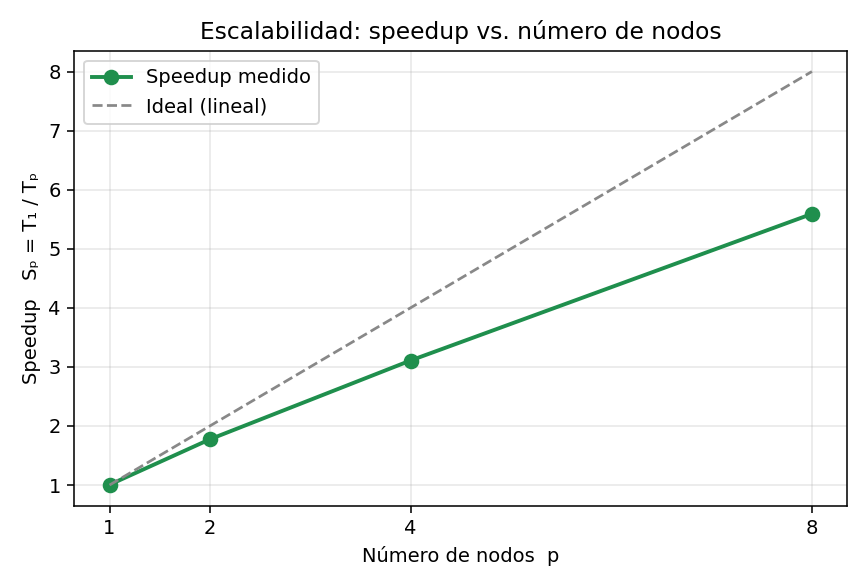
\includegraphics[width=0.49\linewidth]{demo_adsb/results/graficos/speedup.png}\hfill
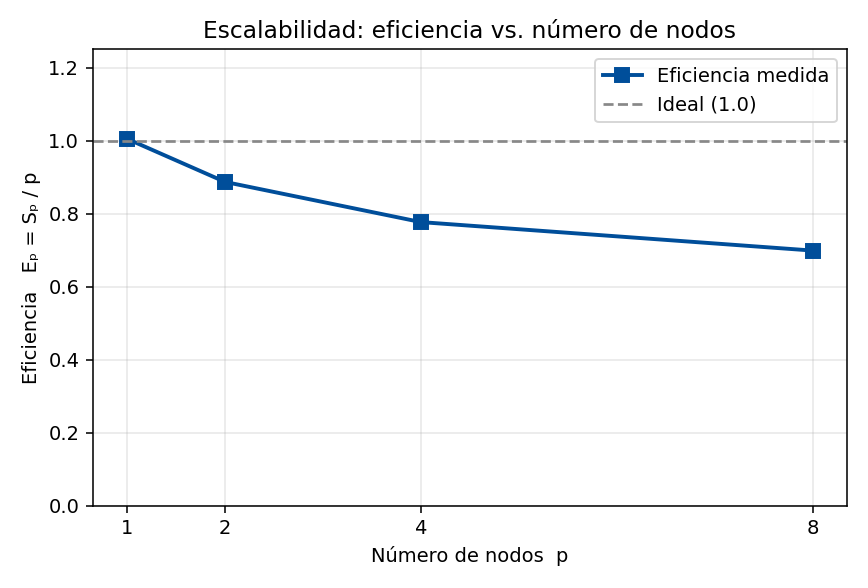
\includegraphics[width=0.49\linewidth]{demo_adsb/results/graficos/eficiencia.png}
\caption{Speedup (izq.) y eficiencia (der.) vs.\ número de nodos $p$. El speedup medido sigue la
tendencia lineal ideal con una separación creciente por \emph{overhead}.}
\label{fig:sp}
\end{figure}

\textbf{Modelo analítico del \emph{overhead}.} Ajustando $T_p \approx T_1/p + o(p)$, el término de
\emph{overhead} $o(p)=p\,T_p-T_1$ crece con $p$ (Cuadro~\ref{tab:esc}), pero su \textbf{costo marginal por
nodo añadido} \emph{decrece} ($1{,}66 \to 1{,}25 \to 0{,}80$~s). La métrica de \textbf{Karp--Flatt}
$e=\dfrac{1/S_p-1/p}{1-1/p}$ estima la fracción serie efectiva:

\begin{table}[H]\centering\small
\caption{Fracción serie efectiva (métrica de Karp--Flatt) calculada desde los speedups medidos.}
\label{tab:kf}
\begin{tabular}{cccc}
\toprule
$p$ & $2$ & $4$ & $8$ \\
\midrule
$e$ (Karp--Flatt) & $0{,}130$ & $0{,}095$ & $0{,}062$ \\
\bottomrule
\end{tabular}
\end{table}

Que $e$ \emph{decrezca} con $p$, en vez de mantenerse constante, indica que la pérdida de eficiencia
\textbf{no} proviene de una región estrictamente secuencial (caso de Amdahl puro), sino de un costo de
coordinación por corrida que se \textbf{amortiza} al crecer el cómputo paralelo: el sistema escala mejor
de lo que predeciría una fracción serie fija.

\textbf{Calidad de la detección (datos reales).} Sobre los 636 vuelos reales, con 12 anomalías inyectadas
para validar (umbral $\sigma\ge 4$), la ejecución distribuida en el \textbf{clúster QEMU (nodo1+nodo2,
4~lotes c/u)} obtuvo:

\begin{table}[H]\centering
\caption{Calidad sobre datos reales (evidencia \texttt{job-20260702-163156}).}
\begin{tabular}{lcl}
\toprule
Métrica & Valor & Significado \\
\midrule
Recall & $\mathbf{1{,}00}$ & anomalías inyectadas detectadas (validación) \\
Hallazgos reales en top-12 & $8$ & vuelos reales genuinamente anómalos \\
precision@12 & $0{,}33$ & top-k inyectadas; el resto son hallazgos reales \\
TP / FP & $12 / 101$ & con la salvedad de que los ``FP'' son vuelos reales raros \\
\bottomrule
\end{tabular}
\end{table}

\textbf{Equivalencia.} En todas las corridas, el ranking y las métricas de la versión distribuida
coincidieron \textbf{exactamente} con la línea base secuencial.

% ===================== 11. ANALISIS =====================
\section{Análisis y discusión}
\textbf{El patrón escala.} La inferencia por particiones es \emph{embarrassingly-parallel}; sin
dependencias entre trozos, el speedup crece casi linealmente hasta que el \emph{overhead} de coordinación
y comunicación se vuelve relevante. La eficiencia baja de $1{,}00$ ($p{=}1$) a $0{,}70$ ($p{=}8$),
consistente con el overhead creciente ($+5{,}6$~s a $p{=}8$): a más nodos, más mensajes y más coordinación
por unidad de cómputo.

\textbf{Granularidad: la variable determinante.} La carga densa escala bien porque cada trozo tiene
suficiente cómputo. En cambio, la variante sobre \textbf{datos reales} (636 vuelos, $\approx$0{,}07~s de
cómputo total) es \textbf{I/O-bound}: la red y la coordinación dominan y el speedup resulta $<1$. Esto
\textbf{no es un fallo} sino la lección clásica de granularidad: paralelizar sólo acelera si las
particiones son suficientemente grandes. Se reporta con honestidad y se separa explícitamente de la
carga densa usada para medir escalabilidad.

\begin{table}[H]\centering\small
\caption{Por qué una misma arquitectura acelera o no: efecto de la granularidad.}
\label{tab:gran}
\begin{tabular}{lccc}
\toprule
Carga & Cómputo por trozo & Transferencia & Resultado ($p{=}8$) \\
\midrule
Densa (semilla) & alto (miles de trayectorias) & $\approx 0$ (sólo semilla) & $S_8=5{,}59$ (acelera) \\
Datos reales (636) & bajo ($\approx 0{,}07$~s total) & dataset por la red & $S_p<1$ (I/O-bound) \\
\bottomrule
\end{tabular}
\end{table}

\textbf{GIL y modelo de procesos.} Al usar agentes-proceso (no hilos) el GIL no limita el cómputo: cada
agente ejecuta en su propio intérprete. El costo es la \textbf{serialización}, mitigada con
\emph{datos-por-semilla}.

\textbf{Tolerancia a fallos.} El sistema completó trabajos con nodos caídos, demostrando que el diseño de
cola dinámica + reintentos + exclusión degrada correctamente ante fallas.

\textbf{Cuellos de botella y límites.} (i) A $p$ alto, la coordinación centralizada en el host limita la
eficiencia. (ii) El volumen de datos reales disponible (una \emph{snapshot}) es pequeño para exhibir
escalado; ampliarlo (o usar el histórico) movería el punto de equilibrio. (iii) El scoring MAD es simple;
un DTW contra rutas canónicas capturaría más tipos de anomalía.

\textbf{Amenazas a la validez.} (i) \emph{Medición de tiempos}: se mitiga con una corrida de calentamiento
descartada, 3~repeticiones y reporte de la desviación (Cuadro~\ref{tab:esc}), que resultó baja
($\le 0{,}05$~s). (ii) \emph{Generalización}: la escalabilidad se mide sobre carga sintética densa y no
sobre el flujo real de bajo volumen; esto se declara explícitamente y no se extrapola. (iii) \emph{Ground
truth}: al ser escaso en datos reales, el recall se mide sobre anomalías \textbf{inyectadas}, por lo que
cuantifica la sensibilidad ante perturbaciones conocidas, no la cobertura de todo tipo de anomalía. (iv)
\emph{Entorno}: un único host físico; en un clúster con red real el \emph{overhead} de comunicación sería
mayor y desplazaría el punto de equilibrio de la granularidad.

% ===================== 12. CONCLUSIONES =====================
\section{Conclusiones}
Se cumplió el objetivo: un orquestador distribuido propio detecta y rankea anomalías ADS-B con evidencia
reproducible. El \textbf{speedup medido} ($S_8=5{,}59$, $E_8=0{,}70$) y la \textbf{equivalencia} exacta
con la línea base defienden la decisión de distribuir, y el \textbf{recall $=1{,}0$} valida la calidad. El
aprendizaje central es que la \textbf{granularidad} decide si distribuir conviene: la misma arquitectura
acelera con cómputo denso y no acelera con datos reales de bajo volumen (I/O-bound). La estrategia
cambiaría al escalar a datos reales masivos, dirección que se detalla en la Sección~\ref{sec:futuro}.

% ===================== TRABAJO FUTURO =====================
\section{Trabajo futuro}\label{sec:futuro}
El prototipo abre líneas concretas de continuación, ordenadas por impacto:
\begin{itemize}[nosep,leftmargin=1.3em]
  \item \textbf{Datos reales masivos}: ingerir el histórico o un flujo continuo de OpenSky desplazaría el
        punto de equilibrio de la granularidad y haría que la variante real también escale, no sólo la
        carga sintética densa.
  \item \textbf{Particionamiento con Dask}: reemplazar la partición manual por colecciones y un
        \emph{scheduler} distribuido facilitaría el balanceo y la ejecución sobre varios hosts físicos.
  \item \textbf{Kernels densos}: vectorizar las \emph{features} (NumPy) o compilar el cálculo por
        trayectoria con \textbf{OpenMP}/\emph{numba} reduciría el costo por trozo y elevaría el techo de
        \emph{speedup}.
  \item \textbf{Modelos de anomalía más ricos}: \emph{Isolation Forest}, \emph{autoencoders} o alineamiento
        \emph{DTW} contra rutas canónicas capturarían tipos de anomalía que el puntaje MAD no separa.
  \item \textbf{Coordinación jerárquica}: para $p$ alto, sub-coordinadores por grupo evitarían el cuello de
        botella de la coordinación centralizada en un único host.
\end{itemize}

% ===================== 13. REFERENCIAS =====================
\section*{Referencias}
\begin{enumerate}[nosep,leftmargin=1.6em]
  \item Grama, A., Gupta, A., Karypis, G., \& Kumar, V. (2003). \textit{Introduction to Parallel Computing} (2nd ed.). Addison-Wesley.
  \item Pacheco, P. (2011). \textit{An Introduction to Parallel Programming}. Morgan Kaufmann.
  \item Tanenbaum, A. S., \& Van Steen, M. (2017). \textit{Distributed Systems} (3rd ed.).
  \item OpenSky Network. \textit{Live API / state vectors}. \url{https://opensky-network.org}
  \item Textualize. \textit{Textual documentation}. \url{https://textual.textualize.io}
  \item Paramiko. \textit{Paramiko (SSH2) documentation}. \url{https://www.paramiko.org}
  \item Python Software Foundation. \textit{Python 3 documentation}. \url{https://docs.python.org/3/}
\end{enumerate}

% ===================== 14. ANEXOS =====================
\section*{Anexos}
\textbf{A. Instrucciones de ejecución.} Instalación, comandos de línea base, ejecución local/clúster,
benchmark y gráficos: \texttt{README.md} (raíz) y \texttt{demo\_adsb/GUIA\_EJECUCION.md}.
\textbf{B. Declaración de uso de IA.} Ver \texttt{anexos/DECLARACION\_USO\_IA.md}: se usó un asistente de
programación (IA generativa) como apoyo; el grupo comprende, validó y defiende todo lo entregado, y toda
medición proviene de ejecuciones reales y trazables (\texttt{demo\_adsb/results/}).
\textbf{C. Evidencia.} Tablas en \texttt{demo\_adsb/results/tablas/} y gráficos en
\texttt{demo\_adsb/results/graficos/}; el detalle teórico del sistema está en \texttt{DOCUMENTACION.md}.

\end{document}
